

\title{GPU-Powered ECDSA Verification for VANET Applications}
\author{  
        Kostas Papagiannopoulos (RU), Arturo Cedillo Torres (TUe), Mathias Morbitzer (RU)\\
                \textbf{Kerckhoff's Institute}       
}
\date{\today}

\documentclass[11pt,twocolumn]{IEEEtran}
\usepackage{hyperref}
\usepackage{graphicx}
\usepackage{amssymb}
\usepackage{amsfonts}
\usepackage{pbox}
\usepackage{rotating}
\usepackage{float}
\usepackage{sidecap}


\begin{document}
\maketitle

\begin{abstract}
\bf{This paper examines the potential of Graphic Processing Units in Vehicular Ad Hoc Network security applications. It presents a low-latency scalar multiplication algorithm for parallel architectures. The algorithm computes
a 224-bit scalar multiplication on curve P-224, using the NVIDIA 525M GT GPU, achieving a minimum latency of 69ms and a maximum throughput of 10039 scalar multiplications/second. In addition, we propose a 2-tier architectural solution for online cryptographic computations using a CPU and a GPU and finally, compare the GPU device to alternative solutions.}
\end{abstract}

\section{Introduction}\label{intro}
Live verification and authentication with the ECDSA algorithm in a vehicular network  is a particularly demanding computational task, both in terms of latency and throughput.
Traditionally, to achieve high performance (throughput in the range of 40Gbps to 4Gbps) and low latency, it is a common practice to use
dedicated hardware in the form of application specific integrated circuits. Moving to the 4Gbps-100Mbps scale, a combination of
CPUs, network processing units and FPGAs are employed and only in the 100Mbps and lower scale, do we consider an x86 CPU~\cite{gpugems}.
The relatively low number of dedicated hardware unit volumes and the additional R\&D costs w.r.t. cryptographic co-processors (usually priced at a few thousand euros) tend to increase the hardware
price and thus, we are encouraged to search for alternative architectures.\\
An alternative candidate that meets such requirements is the Graphics Processing Unit (GPU). Network processing units
and graphical processing units share a set of common characteristics: both are designed to handle highly data-parallel algorithms, since both the network load/streams
and graphics procedures can be divided to smaller sub-procedures that are handled by a large number of of multithreaded processors (another common feature of network and
graphic processing units)~\cite{gpugems, cudaguide}. Last, as
we mentioned, both are designed to handle large data 
flows and thus, to implement a fast interconnection bus between the processing units and the data~\cite{cudaguide}.

\begin{figure}[h!]
\centering
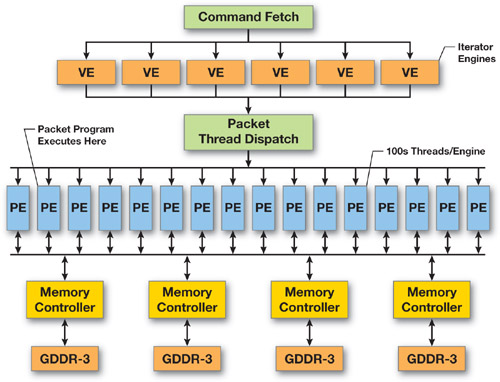
\includegraphics[scale=0.65]{gpu}
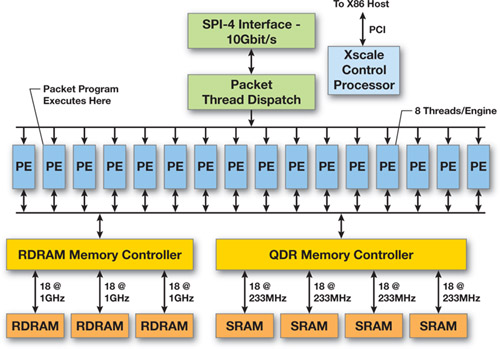
\includegraphics[scale=0.65]{net}
\caption{Top: A modern NVIDIA GPU.
Bottom: Intel Network Processor IXP~\cite{gpugems}.}
\end{figure}
This paper aims at examining and measuring the potential of GPUs when performing live verifications of the ECDSA algorithm in a Vehicular Ad-Hoc Network. Specifically, we will focus on elliptic curve scalar multiplication, i.e. the most computationally intensive part of ECDSA verification and attempt to compute it efficiently with respect to latency (high priority) and throughput (low priority). In sections \ref{vanet}, \ref{crypto} and \ref{cuda} we establish the network context in which we examine the problem, the cryptographic algorithm in use and the hardware architecture that will be employed. In section \ref{implementation} we present our own GPU-based CUDA ECDSA verification implementation and analyze the mathematical and computational optimizations that we have performed. We benchmark our implementation in section \ref{bench} and we continue by proposing an efficient two-tier architecture with respect to optimal hardware usage \ref{arch}. We conclude in section \ref{conclusions}. 

\section{VANET Primitives}\label{vanet}
Vehicular Ad-Hoc Networks (VANETs) and Vehicular Communication (VC) compose a set of emerging technologies. Vehicles and road-side infrastructure units are equipped with on-board sensory,
processing and wireless communication modules and are capable of providing a wide range of applications to enhance transportation safety and efficiency, as well as infotainment~\cite{kargl}. However, this rich set of features, including warnings about environmental hazards (e.g. ice on the pavement), traffic and road conditions (e.g. emergency braking, congestion, or construction sites) or even local (e.g. tourist) information can be vulnerable to several abuses and attacks. A malicious or infected vehicle may transmit false hazard warnings causing unexpected braking in other vehicular nodes or it may masquerade itself as an emergency vehicle causing, similarly, unexpected behavior. Different types of attacks may attempt to track a vehicle's location and infer private information about its driver and passengers~\cite{kargl}. To thwart this large arsenal of vulnerabilities, VANETs have established several security requirements (with respect to authentication, integrity and privacy) and corresponding standards (IEEE 1609.2 standard for VANET communications~\cite{wave}), which are crucial when implementing safety-related vehicular applications such as intersection/forward/work-zone collision warnings or other emergency signals. \\
However, VANETs need to operate under specific restrictions, in a context which is substantially differentiated from traditional networks. Specifically, to support the authentication mechanism (as a VANET security requirement), the IEEE 1609.2 standard for vehicular ad hoc networks proposes the ECDSA algorithm. Still, the processing overhead of the ECDSA signature generation and verification needs to be examined, assessed and adapted in the VANET context, with respect to factors such the algorithm's time complexity, the processing and transfer delay and vehicle distance, speed and density~\cite{petit}. A low-latency ECDSA implementation can decrease the processing delay, fulfill the standard's requirements and enhance the network's capabilities.
\section{Cryptographic Primitives}\label{crypto}
The Elliptic Curve Digital Signature Algorithm (ECDSA)~\cite{certicom} is the elliptic curve variant of the existing Digital Signature Algorithm (DSA)~\cite{dss}. In our discussion we use  the P-224 curve, recommended by NIST\footnote{National Institute of Standards and Technology.}~\cite{dss}, however the mathematical and implementation optimizations presented in section \ref{implementation} apply to the P-256 curve as well.
\subsection{ECDSA Signature Generation \& Verification}\label{signature}
 The P-224\footnote{The exact domain parameters used by P-224 are stated in  \cite{certicom,dss}.} is a curve in short Weierstrass form, namely $y^2=x^3+a*x+b$, over the finite field $\mathbb{F}_q$, $q$ large prime and group order $n$. In P-224 curve there exists a base point $G(xG, yG)$ which is used in generating each private/public key pair $(d,Q)$, where $Q=[d]G$.  To sign a message $m$, the algorithm performs the following steps:
\begin{itemize}
\item The signer selects a random $k, 1\leq k\leq n-1$, the random ephemeral key and calculates the hash value $e$ of the message $m$, $e=H(m)$.
\item He computes $[k]G=(x_1, y_1)$ and $r=x_1$ $mod$ $n$.
\item He calculates $k^{-1}mod$ $n$ and $s = k^{-1}(e+dr)$ $mod$ $n$. The signature on message $m$ is the tuple $(r,s)$.
\end{itemize}
To verify the signature, the verifying party shares the same domain parameters (curve, group) and associated public key $Q$ with the signer. Subsequently:
\begin{itemize}
\item He receives $m$ and $(r,s)$, computes the hash value $e$ of message $m$ and $w=s^{-1}$ $mod$ $n$.
\item $u_1=ew$ $mod$ $n$ and $u_2=rw$ $mod$ $n$.
\item He performs two scalar multiplications, $X=[u_1]G+[u_2]Q$, $X(x_1,y_1)$ and computes $\upsilon=x_1$ $mod$ $n$. He only accepts the signature if $\upsilon=r$.
\end{itemize}
It is already observable that the most computationally demanding part of ECDSA verification is the last step, i.e. the two scalar multiplications~\cite{petit}. Within our scope is to efficiently implement scalar multiplication on the P-224 curve and thusly, provide low-latency ECDSA verification.  
\subsection{ECDSA Security \& Efficiency} \label{security}
The motivation behind an elliptic curve version of DSA were recent advances in number theory, namely the Number Field Sieve~\cite{sieve} and the Baby-Step/Giant Step method~\cite{babystep}. During the DSA domain parameter generation a prime $p$ is chosen, then a large prime $q$ is selected such that $p$ divides $q-1$. Based on this large prime $q$ we generate a group $\mathbb{F^*}_q$ of order $n$. The Number Field Sieve requires $q>2^{1024}$ and the Baby-Step/Giant-Step attack requires $p>2^{160}$ in order for DSA to achieve the rough equivalent of an 80 bit DES~\cite{des} cryptographic strength.\\
In this context, a significant performance penalty is induced: the DSA algorithm only needs a finite abelian group of size $2^{160}$, but the Number Field Sieve forces us to work with group elements of 1024 bits in size.  This issue makes DSA slower even than RSA signatures~\cite{rsa}, e.g. DSA verification requires two exponentiations modulo a 1024-bit number while RSA verification requires only one.\\
However, the elliptic curve version of DSA is not affected by the Number Field Sieve attack due to the non-multiplicative nature of elliptic curves~\cite{koblitz}. Thus, ECDSA can run more efficiently and has smaller footprints and key sizes than almost all other signature schemes. The very small signature footprint (320 bits) and the low number of computations required (2 scalar multiplications) make the ECDSA scheme particularly attractive for VANET applications (such as V2V authentication), where limited bandwidth is commonly encountered.
%\begin{table}[h]
%\small
%\begin{tabular}{| l | c | c| }
   % \hline
   % Algorithm & Signature Size & Verification Cost \\ \hline
   % RSA & 1024 bits & \pbox{30cm}{1 exponentiation ($mod$ $1024$)} \\ \hline
   % DSA & 1024 bits & 2 exponentiations ($mod$ $1024$)\\ \hline
   % ECDSA & 320 bits &  \pbox{20cm}{2 scalar multiplications \\(in field of order $<2^{160}$)}\\
   % \hline
  %\end{tabular}
%\caption{\scriptsize{Signature size (in bits) and computational cost of the RSA, DSA and ECDSA signature schemes. All schemes offer the same security level ($\sim$80 bit DES encryption). The ECDSA signature %consists of $(r,s)$, 160 bits each and only requires 2 scalar multipltications, as seen in section~\ref{signature}.}}
%\label{tab:sizetable}
%\end{table}
%\\


\section{Hardware Primitives}\label{cuda}
Typical V2V communication and authentication scenarios involve the broadcast of a large number of messages and thus, the need to efficiently verify those messages (via low-latency ECDSA verification) before acting based on their content. In order to sucessfully address this engineering challenge, we examine the potential of Graphics Processing Units (GPUs) in this computationally intensive task.\\
General purpose computing on graphics processing units (GPGPU) has managed to transform modern GPUs into highly parallel, multithreaded, multicore processors with impressive computational power and very high memory bandwidth. Modern GPU architecture features a wide data path and a large number of processing units (cores) in order to achieve high data bandwidth and a large level of parallelism~\cite{cudaguide}.\\
To enable these capabilities, NVIDIA introduced the Compute Unified Device Architecture (CUDA)~\cite{cudaguide}: a framework that provides functions to control the GPU from the host. Every CUDA application consists of a serial program running on the CPU (with the common x86 instruction set) and a parallel \emph{kernel}, running on the GPU, on GPU-specific assembly language.\\
This research attempts a high level parallelization of ECDSA verification, i.e. each required scalar multiplication will be assigned to a single thread. Alternative options would be to parallelize the elliptic curve arithmetic (as performed by Joppe W. Bos~\cite{bos}, based on previous work by Fischer et al.~\cite{fischer}).  A typical \emph{kernel} execution involves partitioning our signature set into \emph{threads}, organized in \emph{thread blocks}, transferring signatures to the GPU memory, executing many scalar multiplications in parallel using all the GPU cores and then copying the results back to host memory. This partitioning/organization model can also be seen in figure \ref{cudamodel}.
\begin{figure}
\centering
\includegraphics[scale=0.4]{cudamodel}
\caption{The CUDA kernel (grid), block and thread model~\cite{cudaguide}. Signature batches are partitioned and assigned to CUDA cores. Computations are carried out in the GPU and transfered back to the the host.}
\label{cudamodel}
\end{figure}
\section{ECDSA Implementation \& Optimization}\label{implementation}
For the purposes of fast and efficient ECDSA verification and resultingly scalar multiplication, we have developed the set of all required arithmetic operations, providing mathematical or CUDA-related optimizations when possible (section \ref{core}). Although there exist elliptic curve cryptographic libraries (OpenSSL, Crypto++) some of which have efficient implementations (e.g. MIRACL~\cite{libs}), they have not been ported/adapted to the CUDA model yet. We continue, by providing a full-scale deployment to a GPU and several memory related optimizations (section \ref{deploy}).
\subsection{Core Operations \& Optimizations}\label{core}
In this section, we analyze bottom-up all the required numerical operations, namely, simple field arithmetic (addition, multiplication), modular reduction, elliptic curve arithmetic (coordinates, addition, doubling) and finally, scalar multiplication techniques.
\begin{itemize}
\item \textbf{Addition.} We work on the P-224 curve, so we need to add large integers sized 224 bits each. The multi-precision addition (and similarly subtraction) operation is straightforward: the large 224-bit integer is divided to 7 variables of 32-bits each and 8 32-bit additions are computed. We use the CUDA pseudo-assembly PTX\footnote{The CUDA pseudo-assembly PTX is an assembly-like language focused on cross-GPU compatibility. Below PTX, there exist additional translation layers that are GPU-specific.}  instead of C code in order to facilitate the addition using the native add-with-carry command~\cite{ptxcuda,ptx}. This method gives us the advantage to directly access the carry and not waste memory and computations to keep it in a separate variable in C code.
\small
\begin{verbatim}

add.cc.u32		%a0, %a0, %b0;
addc.cc.u32	%a1, %a1, %b1;
addc.cc.u32	%a2, %a2, %b2;
addc.cc.u32	%a3, %a3, %b3;	
etc.
\end{verbatim}
\normalsize
As shown, we add the two 224-bit integers $a,b$, using  the 32-bit native add command with carry-in and carry-out ($addc.cc$). We store the result in one of the integers, for instance $a$, to consume less memory. 
\item \textbf{Multiplication \& Squaring.} To implement multiplication $a*b$ between 224-bit integers, we represent the integers $a,b$ using 256-bits (i.e. 8*32-bit integer variables). We apply 3 levels of Karatsuba expansion~\cite{karatsuba}, i.e. we transform the 256bit multiplication to 128bit multiplications (and some additions), the 128bit multiplication to 64bit multiplications and finally we reach our basic 32-bit multiplication (similarly to K. Zhao~\cite{zhao}), which is shown below.\\
\small
\begin{verbatim}
mul.lo.u32	 %low32bits, %a, %b;
mul.hi.u32	 %high32bits, %a, %b;
\end{verbatim}
\normalsize
To perform these reductions we use the Karatsuba multiplication algorithm which reduces the multiplication of two $n$-digit numbers to $n^{log_23}$ single-digit multiplications (where schoolbook multiplication reduces to $n^2$ single-digit multiplications). For instance, the 2-digit multiplication $16*42$ can be reduced to $6*2+10*[(1+6)*(4+2)-1*4-6*2]+10^2*(1*4)$, instead of $6*2 + 10*(1*4) + 10*(6*4) + 10^2*(1*4)$. Last, the multiplications and additions required are carried using PTX assembly and the GNU software guidelines~\cite{gnu}. Squaring is performed similarly. We note that that the Montgomery multiplication~\cite{montgomery} method is also a viable alternative to Karatsuba multiplication.
\item \textbf{Modular Reduction.} We have identified two cases of modular reduction. The first case applies to reduction after addition. Adding two 224-bit integers may overflow to a 225-bit integer, thus after each addition/subtraction, we check for overflow and if that is the case, we achieve the modulo reduction simply by adding/subtracting the group order $n$ from the result, depending on the result's sign.\\
The second case applies to reduction after multiplication. Multiplying two 256bit integers yields a result of $2*256-1=511$ bits. There exist several methods for modulo reduction, namely Barrett~\cite{baret} and Montgomery~\cite{montgomery} reduction, with the latter being more efficient. However, based on the findings by Johnson et al.~\cite{modcomparison}, the Montgomery reduction method demonstrates efficiency \emph{after} 1024 bits, which makes it applicable for RSA and not ECDSA implementations. Barrett reduction is still a viable solution, however it is preferable to exploit the special structure of the P-224 curve ($2^{224}-2^{96}+1$) and apply the Special Form Moduli reduction technique~\cite{hac,microsoft}. This technique is applicable only if the modulus $n$ can be re-written in the form: $n=b^t-c$, where c is an $l$-digit base $b$ positive integer and it is shown below.\\
\small
\begin{verbatim}
INPUT: a base b, positive integer x, 
and a modulus n = b^t − c. 

OUTPUT: r = x mod n.
1. q0=x/b^t   
2. r0=x-q0*b^t   
3. r=r0, i=0 
4. While qi > 0 do the following:
	4.1 qi+1= (qi*c)/b^t   
	4.2 ri=qi*c-qi+1 * b^t 
	4.3 i= i + 1, r= r + ri.
5. While r >= n do: r =r - n
6.  Return(r)

\end{verbatim}
\normalsize
For curve P-224, base $b$ is 2, $b^t=2^{224}$ and $c=2^{96}-1$. Steps 1,2 consist of a right and a left shift by 224 bits. In Step 4.1, division by $2^{224}$ is a simple right shift but in order to avoid the multiplication $q_i*c$ we slightly tweak the algorithm and rewrite $q_i*c=q_i*(2^{96}-1)=q_i*2^{96} - q_i $ and thus, it becomes a left shift (96 bits) and a subtraction. We tweak Step 4.2 similarly.
\item \textbf{Elliptic Curve Coordinates.} Inversion of a number in $\mathbb{F^*}_q,q$ large prime can be computationally intensive and even unsuitable for the GPU architecture. Thus, we choose to represent our elliptic curve using projective coordinates as suggested by IEEE standard on public key cryptography~\cite{cryptostandard}. In addition, we exploit the fact that P-224 has parameter $a=-3$ and we use the projective-3 coordinates which allow faster elliptic curve doubling compared to simple projective coordinates~\cite{efd}. Each point $(x,y)$in the elliptic curve is represent as $(X, Y, Z)$, where $x=X/Z$ and $y=Y/Z$.
\item \textbf{Elliptic Curve Addition \& Doubling.} Based on the work by Lange and Bernstein~\cite{scalar}, we implement elliptic curve addition and doubling using the projective-3 formulas. Elliptic curve addition costs 12 field multiplications and 2 field squarings (as described by Cohen, Miyaji, Ono~\cite{cohen}), while elliptic curve doubling costs 7 multiplications and 3 squarings (as described by Bernstein, Lange~\cite{efd}).\\\\
\normalsize
\emph{Addition formula:}
\small
\begin{verbatim}
(X3,Y3,Z3)= (X1,Y1,Z1)+(X2, Y2, Z2)

Y1Z2 = Y1*Z2
      X1Z2 = X1*Z2
      Z1Z2 = Z1*Z2
      u = Y2*Z1-Y1Z2
      uu = u2
      v = X2*Z1-X1Z2
      vv = v2
      vvv = v*vv
      R = vv*X1Z2
      A = uu*Z1Z2-vvv-2*R
      X3 = v*A
      Y3 = u*(R-A)-vvv*Y1Z2
      Z3 = vvv*Z1Z2

\end{verbatim}

\normalsize
\emph{Doubling formula:}
\small
\begin{verbatim}
(X3,Y3,Z3)=[2](X1,Y1,Z1)

w = 3*(X1-Z1)*(X1+Z1)
      s = 2*Y1*Z1
      ss = s2
      sss = s*ss
      R = Y1*s
      RR = R2
      B = 2*X1*R
      h = w2-2*B
      X3 = h*s
      Y3 = w*(B-h)-2*RR
      Z3 = sss

\end{verbatim}
\normalsize
\item \textbf{Scalar Multiplication.} We use the simple method of `double and add' to compute the scalar multiplication on the elliptic curve (shown below), which requires $n$ doublings and $n/2$ additions for an $n$-bit  scalar.\\
\small
\begin{verbatim}
Compute [d]P with the following
representation: 
d= d0+2d1+(2^2)d2+...+(2^m)dm
 1. Q = 0
 2. for i from m to 0 do
     2.1 Q := 2Q (using  doubling)
     2.2 if di = 1 then
	         Q := Q + P (using  addition)
 3. Return Q
\end{verbatim}
\normalsize
More efficient variations exist, such as the addition-subtraction chain proposed by Lange \& Bernstein~\cite{scalar}. Similarly, every ECDSA verification consists of two scalar multiplications and the Shamir trick~\cite{trick} can use precomputations to achieve better computational efficiency. Future work should attempt to implement those techniques in a parallel environment and measure the corresponding benefits. Last, we note that several previous researchers~\cite{bos,fischer,antao} have employed the Montgomery ladder technique~\cite{ladder} to implement scalar multiplication. Their motivation was the resistance versus side-channel attacks offered by this technique. However, since we are solely focusing on the verification side of the ECDSA computations, which is a public process and does not involve secret keys, it is deemed unnecessary for the scope of our work. 
\end{itemize}
\subsection{CUDA Deployment}\label{deploy}
Our strategy to efficiently implement the ECDSA verification is to offload the heavy computational part (i.e. the 2 scalar multiplications) to the GPU. Our implementation parallelizes the ECDSA verification process on client level, i.e. each verification message (which requires 2 scalar multiplications) acquires 2 threads inside the CUDA kernel to perform the multiplications in parallel. Several different grid/block size configurations have been benchmarked and are visible in section \ref{benchmarks} and table \ref{tab:spectable}. Alternative parallelization methods would include parallelization on the elliptic curve or finite field arithmetic and they have the potential of further decreasing the latency at the cost of throughput.\\
Constant variables such as the group order and base points ($xG, yG$) of the elliptic curve are stored in constant memory for faster access. No internal communication is required between threads or blocks so we did not make use of the shared memory.
\section{Benchmarking \& Architecture}\label{benchmarks}
This section benchmarks the performance of our scalar multiplication implementation and based on the metrics, comparisons and additional observations, we discuss potential architectures to efficiently tackle this computational problem.
\subsection{Benchmarking Results}\label{bench}
The benchmarking was performed on a GeForce 525M GT with 96 CUDA cores, processor clock 1200MHz and Fermi architecture (i.e. compatible with CUDA v2 ~\cite{cardspecs}) and can also be viewed in tables \ref{tab:spectable}, \ref{tab:spectable1} and figure \ref{lat}. Our fastest result obtained in 525M  when computing a single 224-bit elliptic curve scalar multiplication, has a latency of 69 milliseconds when dispatching a single thread. \\
The comparison with the related art, namely the experimental results, is not straightforward since different GPU platforms are employed, each one with different architectural and performance characteristics. Still, we attempt to compare our latency results with metrics on relatively similar GPUs in terms of CUDA cores and clock speed. R. Szerwinski and T. Guneysu~\cite{iambetterthanthem} propose several approaches for asymmetric cryptography, namely RSA and EC cryptography on an NVIDIA 8800 GTS GPU (96 CUDA cores, 1200 MHz clock, ranking higher on benchmarks than 525M). The authors' implementation suggest a latency of 305 ms and a throughput of 1412.6  operations/sec. S. Antao, JC. Bajard and L. Sousa~\cite{antao}, when implementing P-224 scalar multiplication on Nvidia 8800 GTS GPU achieved a latency of 30.3 msec (for a single multiplication) and a throughput of 3138 operations/sec. We note that Antao et al. presented an implementation that parallelizes the elliptic curve arithmetic to spread the workload in several threads and thus, reduce the latency. The current state of the art performance is achieved by Joppe Bos~\cite{bos} by reducing the latency to 10 ms until 2 ms for modern Fermi GPUs (GeForce GTX 465, 480, 580) with a large number of cores (240 until 512) and higher clock speeds (from 1476MHz until 1544MHz). The GPU latency results are also visible in Table \ref{tab:spectable}, along with latency results for CPUs.\\ 
High throughput is a less important (compared to low latency), yet desirable capability for VANET and network applications in general. We note that a tradeoff exists between latency and throughput; high throughput translates to large memory transfers from host to GPU and large amount of threads being dispatched to the GPU's streaming multiprocessors. With a latency of 102 milliseconds and a gridsize of 16 (which we found to be optimal w.r.t. throughput/latency - see Table \ref{tab:spectable1}) we achieved a throughput of 10039 scalar multiplications per second on GeForce 525M. We need to stress the fact that the GPU is a \emph{high latency, high throughput} device without many levels of caching and not particularly suited to low-latency applications. Our implementation (as well as other implementations~\cite{bos,antao,iambetterthanthem}) attempt to utilize the high throughput and parallelism to hide the latency issue. However, a CPU is far more suitable for low-latency applications due to its architectural focus on cache hierarchy, and this is viewable on Table \ref{tab:spectable}, where an Intel i7 processor can compute a scalar multiplication in 0.9 msecs. On the other hand, the large cache hierarchy renders it less capable to produce high throughput, resulting in an Intel i7 with throughput of 46176, substantially less than GTX 465,480,580.
\subsection{Discussion on Architecture}\label{arch}
To address the native hardware limitations on CPU (low throughput) and GPU (high latency) we propose a two tier-hardware architecture (figure \ref{2tier}). When constructing an ECDSA verification architecture with cost $C$, the quick option is to invest $C$ in either a GPU or a CPU. Alternatively, the two-tier architecture will invest $C$ distributed in both a GPU and a CPU (ideally by dividing to $C/2$ and $C/2$). When the network traffic is low, the CPU will perform the majority of the work at a low latency. When traffic increases, thus rendering the CPU unable to handle the high load in a timely manner, the CPU will offload scalar multiplications to the GPU, where the latency is higher but throughput and parallel processing capabilities are substantially improved; slow operations such as the inversion step before scalar multiplication can remain in the CPU. This approach has also been proposed for similar tasks, e.g. a dedicated cryptographic server for online encryption/decryption in the  SSL/HTTPS software suites~\cite{kaist}. A similar -but inversed- two-tiered approach was also followed by G. Vasiliadis and S.Ioannidis~\cite{gravity} when using the GPU as \emph{first filter} in malware detection. The GPU attempts to rule out a large portion of the traffic on its own (exploiting its large parallel processing potential) and then transfer the remaining potential threats to the CPU for postprocessing.\\
\begin{figure}
\centering
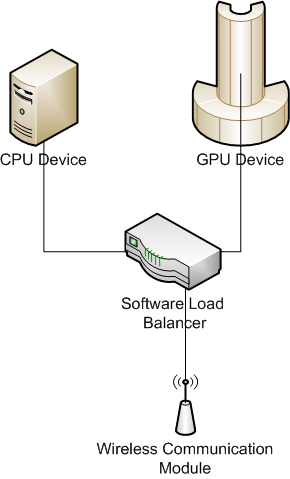
\includegraphics[scale=0.45]{2tier}
\caption{A two-tier processing architecture. Incoming packets from the wireless network are being balanced and distributed between CPU and GPU, according to the traffic load.}
\label{2tier}
\end{figure}
Another issue that can affect the architecture is the computational bottlenecks which was encountered in two forms.  The first type of bottleneck is a native performance issue of GPUs: their global memory is limited and the data they are able to process is upper-bounded by the global memory offered~\cite{cudaguide}. The common programming practice is to make subsequent kernel calls in the device, trying to allocate as much memory as possible in every call, due to the high penalty of data transfers between CPU host memory and GPU device memory. In general, this type of bottleneck will not be especially harmful due to the fact that our main objective is latency and not huge throughput. The second case of bottleneck is more generic. Researchers that employed GPUs to perform `live' operations such as live encryption/decryption for ssl/https purposes~\cite{kaist} have observed that network packet queuing and processing may be delayed even by the Linux kernel handling procedures. To tackle these issue and to demonstrate the construction of a large-scale GPU-assisted `live' operation system, researchers have created specific network architectures, manipulating the Linux kernel, its networking interfaces/queues and ensuring traffic load balancing~\cite{midea}.
\begin{figure}
\centering
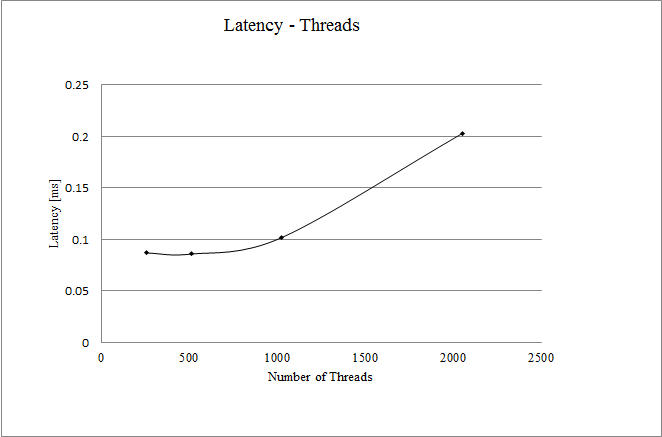
\includegraphics[scale=0.35]{latencygraph.png}

\caption{Latency vs. Throughput tradeoff graph. Figure demonstrates
 the latency penalties incurred by increasing blocksize for constant gridsize equal to 16.}
\label{lat}
\end{figure}
\section{Conclusions}\label{conclusions}
The constant evolution of VANETs gave rise to the need for high computational power on every vehicular node. The GPU is an affordable device that has been deemed capable performing security-related computational tasks with low latency and high throughput. Still,it comes with several advantages and disadvantages compared to other solutions. On the positive side, the GPU is an efficient, high throughput device with little or small R\&D cost related to it; its computational capabilities are constantly improving without any penalty. Thus, they are substantially cheaper compared to a dedicated, custom made crypto-accelerator. On the other hand, they consume a very large amount of energy resources (especially compared to FPGAs), they lack the customization of a dedicated processor and have several issues regarding latency. Moreover, they present substantial issues when processing secret keys due to their vulnerability to memory and cold boot attacks. Whether they will step in the place of specialized hardware will largely depend on the specific application context and adaptability to the new VANET environment. \\
With regards to the computational part of this research, we suggest future work in the following areas: parallelization of the elliptic curve arithmetic on large finite fields including the addition chain improvements and second, parallelization on the finite field arithmetic, where potential for low-latency is larger but thread communication more difficult. Deep inspection of these areas will examine the tradeoff between latency and throughput and deduce the optimal solution, based on specific application requirements.
\onecolumn
\begin{table}
\small
\centering
\begin{tabular}{ l | c | c | c| | c |c }
  
    Ref & Platform & Cores &Processor Clock (MHz) & Min Latency [ms]& Max Throughput [op/sec]\\ \hline
    \cite{iambetterthanthem}  & 8800 GTS & 96 & 1200 &  305.0 & 1413 \\ \hline
    Ours & 525M GT &  96 & 1200 &  69.0 & 10039 \\ \hline
    \cite{antao} &   8800 GTS & 96 & 1200 &  30.3 & 3138 \\ \hline
    \cite{bos} &  465 GTX & 352 & 1215 & 2.6 & 152023 \\
 \cite{bos} &  480 GTX & 480 & 1401 & 2.3 & 237415 \\
\cite{bos} &  580 GTX & 512 & 1544 & 1.9 & 290535  \\

 \hline
\cite{kasper} &  Intel Core i7 & 4 & 3400 & 0.09 & 46176  \\
  \end{tabular}
\caption{\footnotesize{Performance comparison of 224-bit elliptic curve scalar multiplication on different GPU and CPU platforms. Minimum latency achieved is displayed w.r.t. a single scalar multiplication. Maximum throughput is expressed in scalar multiplications per second.}}
\label{tab:spectable}

\small

\begin{tabular}{ l | c | c| | c | c  }
  
    Number of blocks
 & Threads per block
 & Total threads
 &Latency [ms] & Throughput [op/sec]\\ \hline
  
16 & 16 & 256
 & 0.087
 & 2942  \\


16 & 32 & 512
 & 0.086
 & 5953  \\

16 & 64 & 1024
 & 0.102
 & 10039  \\

16 & 128 & 2048
 &0.203
 & 10088


  \\


 \hline
32 & 8 & 256
 & 0.175
 & 1462


  \\
32 & 16 & 512
 &0.173

 & 2959


  \\
32 & 32 & 1024
 & 0.172

 & 5953

  \\
32 & 64 & 2048
 &0.204

 & 10039


  \\

 \hline

64 & 4 & 256
 & 0.350

 & 731
  \\
64 & 8 & 512
 &0.348

 & 1471

  \\
64 & 16 & 1024
 & 0.347

 & 2951

  \\
64 & 32 & 2048
 & 0.345

 & 5936
  \\

 \hline
  \end{tabular}

\caption{\footnotesize{Latency and throughput results for different CUDA kernel configurations. Optimal results w.r.t. latency and throughput were achieved in GeForce 525M with 16 blocks and 32 threads.}}
\label{tab:spectable1}

\end{table}



\twocolumn


\bibliographystyle{abbrv}

\begin{thebibliography}{9}

\bibitem{gpugems}
  E.Seamans, T.Alexander. NVIDIA. 
  \emph{GPU Gems 3, Chapter 35, Fast Virus Signature Matching on the GPU}.
  URL: \url{http://http.developer.nvidia.com/GPUGems3/gpugems3_part01.html}.
 Date Retrieved: 8/2012

\bibitem{kargl}
P. Papadimitratos, L. Buttyan, T. Holczer, E. Schoch, J. Freudiger, M. Raya, Z. Ma, F. Kargl, A. Kung, J.P. Hubaux.
\emph{Secure Vehicular Communication
Systems: Design and Architecture}. Communications Magazine, IEEE, Volume: 46  , Issue: 11 
Page(s): 100-109. 2008.

\bibitem{petit}
J. Petit.
\emph{Analysis of ECDSA Authentication Processing in
VANETs}. 3rd International Conference on New Technologies, Mobility and Security (NTMS). 2009.

\bibitem{bos}
Joppe W. Bos.
\emph{Low-Latency Elliptic Curve Scalar Multiplication. } International Journal of Parallel Programming, Pages 532-550, Volume 40, Number 5. 2012.

\bibitem{fischer}
W. Fischer, C. Giraud, E.W. Knudsen, J.P. Seifert.
\emph{Parallel scalar multiplication on general
elliptic curves over Fp hedged against Non-Differential Side-Channel Attacks.}


\bibitem{ladder}
K. Okeya and K. Sakaurai. \emph{Power Analysis breaks Elliptic Curve cryptosystems
even secure against the timing attacks.} INDOCRYPT 2000, Springer LNCS, pp.
178-190, 2000.

\bibitem{trick}
B. Moller.
\emph{Algorithms for multi-exponentiation}. 2001.

\bibitem{cardspecs}
NVIDIA GeForce 525M Technical Specifications. URL:\url{http://www.geforce.com/hardware/desktop-gpus/geforce-gt-525m/specifications}

\bibitem{ptxcuda}
NVIDIA Compute, PTX:  Parallel Thread Execution. ISA Version 1.4. 2009.

\bibitem{ptx}
Using Inline PTX Assembly In CUDA. 2011.

\bibitem{certicom}
D. Johnosn, A. Menezes, S. Vanstone.
\emph{The Elliptic Curve Digital Signature Algorithm (ECDSA).}
Certicom Research, Canada, Dept. of Combinatorics \& Optimization, University of Waterloo, Canada.

\bibitem{dss}
FIPS PUB 186-3, Digital Signature Standard (DSS).
National Institute of Standards and Technology, Information Technology Laboratory. 2009.

\bibitem{iambetterthanthem}
R. Szerwinski, T. Guneysu. \emph{Exploiting the power of GPUs for asymmetric cryptography}. CHES 2008.

\bibitem{sieve}
C. Pomerance. \emph{A Tale of Two Sieves.} Notices of the AMS 43 (12): pp. 1473–1485. 1996.
\bibitem{babystep}
H. Cohen. \emph{A course in computational algebraic number theory.} Springer. 1996.
\bibitem{des}
FIPS PUB 46-3, Data Encryption Standard (DES).
National Institute of Standards and Technology. 1999.
\bibitem{rsa}
L. Ronald, A. Shamir, L. Adleman.  U.S. Patent 4,405,829. 1977.
\bibitem{koblitz}
N. Koblitz. \emph{Elliptic curve cryptosystems.} Mathematics of Computation 48 (177): 203–209. 1987.
\bibitem{cudaguide}
NVIDIA CUDA C Programming Guide. Version 4.2. 2012.
\bibitem{libs}
A. Abusharekh, K. Gaj. \emph{Comparative Analysis of Software Libraries
for Public Key Cryptography. }ECRYPT Workshop on Software
Performance Enhancement for Encryption and Decryption, pp. 1-16.
2007.
\bibitem{karatsuba}
A. Karatsuba, Yu. Ofman. \emph{Multiplication of Many-Digital Numbers by Automatic Computers.} Proceedings of the USSR Academy of Sciences 145: 293–294. 1962.
\bibitem{montgomery}
Peter Montgomery. \emph{Modular Multiplication Without Trial Division.} Math. Computation, vol. 44, pp. 519–521. 1985.
\bibitem{zhao}
K. Zhao.\emph{ Implementation of Multiple-precision Modular Multiplication on GPU.}

\bibitem{gnu}
Karatsuba Multiplication Guidelines. GNU. URL:\url{http://www.gnu.org/software/gmp/manual/html_node/Karatsuba-Multiplication.html}.
Retrieved: 10/2012.

\bibitem{baret}
P.D. Barrett. \emph{Implementing the Rivest Shamir and Adleman Public Key Encryption Algorithm on a Standard Digital Signal Processor.} Advances in Cryptology CRYPTO'86, Springer. 1986

\bibitem{modcomparison}
M. Johnson, B. Phung, T. Shackelford, S. Rueangvivatanakij.\emph{Modular Reduction of Large Integers Using Classical, Barrett, Montgomery Algorithms. }

\bibitem{efd}
T. Lange, D.J. Bernstein. Explicit Formular Database. URL:\url{http://www.hyperelliptic.org/EFD/g1p/auto-shortw-projective-3.html#addition-add-1998-cmo-2}. Retrieved: 10/2012.

\bibitem{cryptostandard}
IEEE Standard Specifications for Public-Key Cryptography. Microprocessor Standards Committee. 2000.

\bibitem{wave}
IEEE 1609.2 -2006- Trial Use Standard for Wireless Access in Vehicular Environments (WAVE) - Security Services for Applications and Management Messages.

\bibitem{antao}
S. Antao, JC .Bajard, L. Sousa. \emph{ Elliptic curve point multiplication on GPUs. }
Application-specific Systems Architectures and Processors (ASAP), pp. 192-199. 2010.

\bibitem{kasper}
E. Kasper. \emph{Fast elliptic curve cryptography in OpenSSL}. 2nd Workshop on Real-Life Cryptographic Protocols and Standardization. 2012.

\bibitem{hac}
A. Menezes.
Handbook of Applied Cryptography, Chapter 14: Cryptographic Implementations.


\bibitem{scalar}
D.J. Bernstein, T. Lange.
\emph{Analysis and optimization of elliptic-curve single-scalar multiplication.}
 In the proceedings of Fq8. 2008.

\bibitem{microsoft}
T. Acar, D. Shumow.
\emph{Modular Reduction without Pre-Computation for Special Moduli.}Extreme Computing Group, Microsoft Research.

\bibitem{cohen}
H. Cohen, A. Miyaji, T. Ono.
\emph{Efficient elliptic curve exponentiation using mixed coordinates.} ICICS '97 Proceedings of the First International Conference on Information and Communication Security
Pages 282-291. 1997.

\bibitem{midea}
G.Vasiliadis, M.Polychronakis, S.Ioannidis.
\emph{MIDea: A Multi-Parallel Intrusion Detection Architecture.}  Proceedings of the 18th ACM conference on Computer and communications security Pages 297-308. 

\bibitem{cudaguide}
NVIDIA CUDA C Programming Guide. Version 4.2. Date: 4/2012.

\bibitem{kaist}
K.Jang, S.Han, S.Han, S.Moon, K.Park.
\emph{Accelerating SSL with GPUs}.
Dep. of Electrical Engineering, KAIST. Proceedings of the ACM SIGCOMM 2010 conference, Pages 437-438.

\bibitem{gravity}
G.Vasiliadis, S.Ioannidis.
Intistitute of Computer Science, Foundation for Research and Technology - Hellas.
\emph{GrAVity: A Massively Parallel Antivirus Engine}. RAID'10 Proceedings of the 13th international conference on Recent advances in intrusion detection, Pages 79-96. 2010.


\end{thebibliography}
\end{document}







